%% ===================================================================
%% SPICSCON 2026 draft — Meta-Learning for Rapid Personalization of
%% ErrP-Driven BCIs.  IEEEtran conference template.
%%
%% Compile on Overleaf with: Menu -> Compiler -> pdfLaTeX
%% (BibTeX runs automatically on Overleaf for the \bibliography command.)
%% ===================================================================
\documentclass[conference]{IEEEtran}
\IEEEoverridecommandlockouts

\usepackage{cite}
\usepackage{amsmath,amssymb,amsfonts}
\usepackage{graphicx}
\usepackage{booktabs}
\usepackage{xcolor}
\usepackage{url}
\usepackage[hidelinks]{hyperref}

% Nicer table spacing
\renewcommand{\arraystretch}{1.15}

% Relax float placement so full-width figures pack at page tops cleanly
\setcounter{topnumber}{2}
\setcounter{totalnumber}{4}
\setcounter{dbltopnumber}{2}
\renewcommand{\topfraction}{0.92}
\renewcommand{\dbltopfraction}{0.92}
\renewcommand{\textfraction}{0.08}
\renewcommand{\floatpagefraction}{0.7}
\renewcommand{\dblfloatpagefraction}{0.7}

\begin{document}

\title{Meta-Learning for Rapid Personalization of\\Error-Related Potential Brain-Computer Interfaces:\\A Cross-Dataset Benchmark}

\author{
\IEEEauthorblockN{Md Shahidul Islam Dipu, Barshon Sen}
\IEEEauthorblockA{\textit{Department of Computer Science and Engineering}\\
\textit{Rajshahi University of Engineering and Technology}\\
Rajshahi, Bangladesh\\
shahidul03579@gmail.com, sen.barshon@gmail.com}
}

\maketitle

% ===================================================================
\begin{abstract}
When a brain-computer interface (BCI) makes a mistake, the user's
electroencephalogram (EEG) carries a tell-tale error-related potential (ErrP)
that the system can use to detect and correct itself. The difficulty is that
ErrPs look different from one person to the next, so a fresh user typically has
to sit through a long calibration session before the decoder is any good. We ask
whether meta-learning can shorten that session. Instead of fitting a separate
model per user, a meta-model learns an initialization across users that a new
user can fine-tune from only a few trials. We compare ten approaches under one
leave-one-subject-out (LOSO) protocol on two independent ErrP datasets: three
gradient-based meta-learners (MAML, ANIL, Reptile), two metric-based ones
(Prototypical and Matching networks), a subject-conditioned encoder built on
feature-wise linear modulation (FiLM), and four classical baselines (a supervised
MLP, EEGNet, and two Riemannian methods), plus two transfer controls that share
the source-subject data. At a five-trial calibration budget, the gradient-based
meta-learners, the FiLM encoder, and a source-pretrained EEGNet all significantly
improve balanced accuracy over a from-scratch supervised baseline on both datasets
(paired Wilcoxon at the subject level, $N{=}16$, BH-FDR $p<0.05$, large effect).
On the cross-dataset validation paradigm the gradient meta-learners additionally
outperform EEGNet by 6--7 points at $K{=}5$, though this edge closes by $K{=}10$.
Crucially, they also surpass transfer baselines that pretrain on the same source
subjects with the same class-weighted loss, indicating the gain stems from the
episodic meta-objective rather than from data access or imbalance handling.
Ablations show that class-weighted episodic loss is the most important design
choice, while FiLM conditioning and higher feature dimensionality contribute
little. We frame the result as improved low-data personalization, not a
deployment-ready decoder.
\end{abstract}

\begin{IEEEkeywords}
brain-computer interface, error-related potential, meta-learning, few-shot
learning, EEG, personalization
\end{IEEEkeywords}

% ===================================================================
\section{Introduction}
A brain-computer interface (BCI) turns EEG into commands, and like any decoder it
sometimes gets them wrong. When it does, for instance when a P300 speller picks
the wrong letter, the user's brain reacts with a stereotyped \emph{error-related
potential} (ErrP): a fronto-central deflection with an early negativity around
250\,ms and a later positivity around 320\,ms after the erroneous
feedback~\cite{chavarriaga2010learning,spuler2015error}. If the system can read
that signal, it can undo the mistake on its own, with no extra effort from the
user~\cite{iturrate2015teaching}.

Calibration is what stands in the way. Because ErrP morphology shifts with
anatomy, electrode placement, and signal quality, a decoder trained on one person
transfers poorly to the next, and the usual remedy is to record tens of minutes
of labelled trials from every new user before the system works. That per-user
overhead is a large part of why ErrP-BCIs rarely leave the
lab~\cite{yasemin2023single}.

Meta-learning offers a way around it. Rather than learning one decoder per user,
a meta-model trained across many users learns an initialization that adapts to a
new user from a handful of trials~\cite{finn2017model}. We put this idea to the
test and report three things:
\begin{itemize}
\item a head-to-head benchmark of ten personalization methods---three gradient
meta-learners, two metric meta-learners, a subject-conditioned FiLM encoder, and
four classical baselines---all evaluated under one leave-one-subject-out protocol;
\item cross-dataset validation on two structurally different ErrP paradigms,
where the advantage replicates and stays stable across three random seeds; and
\item ablations that pin down which design choices actually carry the result.
\end{itemize}
We are not proposing a new algorithm. The value here is the benchmark, the
cross-dataset evidence, and the analysis of what makes few-shot ErrP decoding work.

% ===================================================================
\section{Related Work}
\textbf{ErrP detection.} ErrPs have been used both to correct BCI output and to
supply reward signals to autonomous agents~\cite{chavarriaga2010learning,iturrate2015teaching}.
Detecting them in a single trial is still hard. Recent surveys weigh linear
discriminants, support-vector machines, and Riemannian classifiers against one
another, and they keep returning to the same two practical issues: preprocessing
choices and the heavy class imbalance of ErrP data~\cite{yasemin2023single,spuler2015error}.

\textbf{Meta-learning.} MAML learns an initialization that adapts in a few
gradient steps~\cite{finn2017model}; ANIL shows that adapting only the classifier
head usually suffices~\cite{raghu2020rapid}; and Reptile reaches a similar place
with first-order updates alone~\cite{nichol2018first}. The metric-based
alternatives, Prototypical~\cite{snell2017prototypical} and Matching
networks~\cite{vinyals2016matching}, instead classify by similarity in a learned
embedding. Feature-wise linear modulation (FiLM) conditions a network on side
information~\cite{perez2018film}; we use it to condition on a subject's support set.

\textbf{Meta-learning for EEG.} Most prior EEG work targets motor imagery: MAML
and relatives for cross-subject decoding~\cite{duan2020meta,an2020fewshot}, and
meta-learned representations for zero-calibration use~\cite{han2024metaeeg}.
Few-shot EEG classification has grown into an active subfield~\cite{wei2024harnessing}.
Single-trial ErrP personalization has received far less attention, and we are not
aware of prior work that validates it across datasets. That is the gap we address.

% ===================================================================
\section{Methods}

\subsection{Datasets}
We use two independent ErrP datasets. The \textbf{primary} dataset is the INRIA
BCI Challenge (NER~2015) P300 speller (16 subjects, feedback-locked ErrP
paradigm)~\cite{perrin2012objective}. The \textbf{validation} dataset is the
ErrP-Coadaptation corpus~\cite{ehrlich2018human}; we use all 16 subjects in the
public release (indexed S03--S18) with no exclusions of our own. It is an
observation-ErrP paradigm in which a participant infers a robot's intended object
from its gaze. The two paradigms differ in task, montage, and stimulus timing,
so consistent results across them indicate transfer across paradigms, not merely
across subjects.

\subsection{Preprocessing}
We applied a 4th-order zero-phase Butterworth bandpass (1--40\,Hz) to the
continuous EEG before epoching to avoid edge artifacts. The INRIA recordings are
sampled at 200\,Hz; the coadaptation recordings at 250\,Hz, where a 50\,Hz notch
was applied before the bandpass to suppress line noise (for the 200\,Hz INRIA data
the 40\,Hz low-pass already removes the 50\,Hz line component, so no separate notch
is used). No resampling was performed; each method's time-domain sizes follow the
native rate. Epochs were cut from $-200$ to $+600$\,ms relative to feedback onset;
per-epoch per-channel baseline correction was applied over $[-200,0]$\,ms; epochs
exceeding $\pm100\,\mu$V peak-to-peak were rejected, and $K$ refers to clean trials
after rejection. Epoch--label alignment used the feedback index to prevent silent
offset errors. The gradient and metric meta-learners operate on the flattened
filtered waveform reduced to 32 whitened principal components (PCA fit on training
subjects only within each fold to prevent leakage); EEGNet and the Riemannian
methods operate on the raw filtered epochs. This input asymmetry follows each
method family's standard usage but is a confound for cross-family comparison; the
feature-representation ablation (Sec.~V) addresses it by varying the PCA
dimensionality, and ``raw'' there denotes the flattened waveform at a higher PCA
rank rather than the time-domain tensor fed to EEGNet.

\subsection{Personalization methods}
We compare, under a $K$-shot protocol ($K$ clean trials from the new user):
\textbf{Full-MAML}~\cite{finn2017model}, \textbf{MAML-ANIL}~\cite{raghu2020rapid},
and \textbf{Reptile}~\cite{nichol2018first} (gradient-based);
\textbf{Prototypical}~\cite{snell2017prototypical} and
\textbf{Matching}~\cite{vinyals2016matching} networks (metric-based); and
\textbf{SubjectConditioned}, an encoder that computes error/correct prototypes
from the support set and modulates a feature extractor via
FiLM~\cite{perez2018film}. All episodic losses are class-weighted (inverse class
frequency) to handle the $\sim$75/25 correct/error imbalance.

\subsection{Baselines}
\textbf{Supervised}: a three-layer MLP (128-64-2 units, LayerNorm, GELU,
Dropout 0.3) trained from scratch on $K$ trials with early stopping, using a
class-weighted loss. It is the only method that does \emph{not} see source-subject
data.
\textbf{EEGNet}~\cite{lawhern2018eegnet}: a compact depthwise-separable CNN whose
backbone is pretrained on the $N{-}1$ source subjects with a class-weighted
cross-entropy loss, then frozen; an $\ell_2$-regularized logistic-regression probe
(class-balanced, lbfgs) is fit on the $K$ support embeddings. EEGNet is therefore
itself a source-pretrained transfer baseline with the same data access as the
meta-learners, not a from-scratch method.
\textbf{Riemannian}~\cite{barachant2012multiclass} and \textbf{Covariance
Alignment}~\cite{barachant2013classification,zanini2018transfer}: covariance-based
classifiers on the SPD manifold.
To further isolate the meta-learning objective from data access, we add two
\emph{fair-transfer} baselines that see exactly the same $N{-}1$ source subjects:
\textbf{Pretrain-FT} pretrains the same MLP backbone on all source subjects with
the \emph{same} class-weighted loss used by the meta-learners, freezes it, and
fits a class-balanced logistic-regression probe on the $K$ new-user trials;
\textbf{Pretrain-ZeroShot} keeps that pretrained backbone and its source-trained
head and applies no new-user adaptation at all. Because these baselines match the
meta-learners on both data access and class weighting, the remaining gap isolates
the episodic meta-objective.

\subsection{Implementation details}
MAML: inner LR 0.01, 5 inner steps, outer LR 0.001 (Adam, weight decay
$10^{-4}$). ANIL: same, inner loop on head only. Reptile: 5 inner steps,
outer step 0.1. SubjectConditioned: 32-dim subject embedding from the
prototype trio, FiLM $\gamma/\beta$ from an embedding MLP. Meta-training runs
2000 meta-iterations with a meta-batch of 4 subjects; each episode is balanced
with 10 support and 40 query trials (5/20 per class). Test-time adaptation uses
5 inner steps and is averaged over 10 evaluation episodes per $K$. The INRIA
recordings are sampled at 200\,Hz and the coadaptation recordings at 250\,Hz, so
EEGNet's temporal kernel length ($f_s/2$) is 100 and 125 samples respectively.
PCA retains 32 whitened components, fit per fold on the training subjects only.
Code, trained per-fold checkpoints, and the exact preprocessing/episode
configuration (including the per-fold retained PCA variance) are released
(anonymized for review): \url{https://anonymous.4open.science/r/errp-meta}.

\subsection{Protocol and statistics}
We evaluate LOSO across all subjects, with three random seeds (42, 123, 456)
and $K\in\{5,10,20\}$. We report balanced accuracy and AUROC, both robust to the
class imbalance, as mean\,$\pm$\,std over the three seeds. We do not tabulate F1:
binary F1 depends on which class is labelled positive (the two corpora use opposite
codings) and rewards majority-class prediction---e.g.\ the majority-predicting
Pretrain-ZeroShot attains a high binary F1 despite near-chance balanced
accuracy---so it is misleading here; the error class is the minority in both
corpora (prior $\sim$0.32 INRIA, $\sim$0.20 coadaptation). The unit of analysis
for inference is the \emph{subject}: under LOSO the three seeds are repeated
measurements of the same 16 held-out subjects, not independent samples, so we
first average each subject's score across seeds and run paired Wilcoxon
signed-rank tests at $N=16$ (exact null distribution). We apply Benjamini--Hochberg
false-discovery-rate (FDR) correction across all pairwise comparisons within each
dataset and report the rank-biserial effect size $r=Z/\sqrt{N}\in[-1,1]$. With
$N=16$ the smallest attainable two-sided exact $p$ is $2/2^{16}\approx3.1\times10^{-5}$;
we report values at this floor as such rather than extrapolating a normal tail.

% ===================================================================
\section{Results}

\begin{table}[t]
\caption{Primary dataset (INRIA NER 2015): balanced accuracy at
$K\in\{5,10,20\}$ and AUROC at $K{=}5$, mean\,$\pm$\,std over three seeds, LOSO
($N{=}16$ subjects). ${\dagger}$ significantly better than Supervised at $K{=}5$
(paired Wilcoxon on per-subject means, BH-FDR $p<0.05$). ${\ddagger}$ not
significantly different from EEGNet at $K{=}5$. EEGNet overtakes the
meta-learners at $K{=}10$--$20$.}
\label{tab:primary}
\centering
\begin{tabular}{lcccc}
\toprule
Method & $K{=}5$ & $K{=}10$ & $K{=}20$ & AUROC \\
\midrule
EEGNet$^{\dagger}$              & $0.600 \pm .009$ & $0.628 \pm .004$ & $\mathbf{0.645} \pm .011$ & 0.640 \\
Reptile$^{\dagger\ddagger}$    & $0.594 \pm .002$ & $0.600 \pm .003$ & $0.607 \pm .003$ & 0.637 \\
Subj.-Cond.$^{\dagger\ddagger}$ & $0.584 \pm .007$ & $0.584 \pm .009$ & $0.587 \pm .013$ & 0.617 \\
Full-MAML$^{\dagger\ddagger}$  & $0.584 \pm .009$ & $0.590 \pm .011$ & $0.590 \pm .008$ & 0.625 \\
MAML-ANIL$^{\dagger\ddagger}$  & $0.581 \pm .013$ & $0.580 \pm .015$ & $0.585 \pm .015$ & 0.614 \\
Prototypical                   & $0.536 \pm .005$ & $0.553 \pm .009$ & $0.569 \pm .002$ & 0.548 \\
Matching                       & $0.535 \pm .002$ & $0.527 \pm .003$ & $0.542 \pm .022$ & 0.546 \\
Cov.\ Align.                   & $0.526 \pm .026$ & $0.546 \pm .025$ & $0.562 \pm .020$ & 0.524 \\
Riemannian                     & $0.517 \pm .015$ & $0.561 \pm .026$ & $0.541 \pm .040$ & 0.542 \\
\midrule
Pretrain-ZeroShot              & $0.563 \pm .007$ & $0.563 \pm .007$ & $0.563 \pm .007$ & 0.601 \\
Pretrain-FT                    & $0.537 \pm .014$ & $0.542 \pm .012$ & $0.544 \pm .018$ & 0.563 \\
\textbf{Supervised}            & $0.527 \pm .034$ & $0.563 \pm .015$ & $0.577 \pm .004$ & 0.538 \\
\bottomrule
\end{tabular}
\end{table}

\begin{table}[t]
\caption{Cross-dataset validation (ErrP-Coadaptation): balanced accuracy at
$K\in\{5,10,20\}$ and AUROC at $K{=}5$, mean\,$\pm$\,std over three seeds, LOSO
($N{=}16$ subjects). ${\dagger}$ significantly better than Supervised at $K{=}5$
(BH-FDR $p<0.05$). At $K{=}5$ the gradient meta-learners also beat EEGNet
(all $r{=}1.0$); at $K{=}10$--$20$ they do not differ significantly from EEGNet,
which is the top method at $K{=}20$. Bold = best at that $K$.}
\label{tab:validation}
\centering
\begin{tabular}{lcccc}
\toprule
Method & $K{=}5$ & $K{=}10$ & $K{=}20$ & AUROC \\
\midrule
Reptile$^{\dagger}$            & $\mathbf{0.720} \pm .003$ & 0.724 $\pm$ .005 & 0.731 $\pm$ .006 & 0.799 \\
Subj.-Cond.$^{\dagger}$        & $0.721 \pm .006$ & 0.724 $\pm$ .004 & 0.723 $\pm$ .008 & 0.800 \\
MAML-ANIL$^{\dagger}$          & $0.717 \pm .001$ & 0.720 $\pm$ .001 & 0.722 $\pm$ .001 & 0.799 \\
Full-MAML$^{\dagger}$          & $0.716 \pm .003$ & 0.720 $\pm$ .001 & 0.724 $\pm$ .001 & \textbf{0.801} \\
Prototypical$^{\dagger}$       & $0.681 \pm .007$ & \textbf{0.727} $\pm$ .002 & 0.732 $\pm$ .008 & 0.744 \\
EEGNet$^{\dagger}$             & $0.654 \pm .004$ & 0.713 $\pm$ .009 & $\mathbf{0.749} \pm .003$ & 0.734 \\
Matching$^{\dagger}$           & $0.650 \pm .009$ & 0.674 $\pm$ .006 & 0.678 $\pm$ .013 & 0.692 \\
\midrule
Pretrain-ZeroShot$^{\dagger}$  & $0.700 \pm .001$ & 0.700 $\pm$ .001 & 0.700 $\pm$ .001 & 0.767 \\
Pretrain-FT                    & $0.590 \pm .021$ & 0.643 $\pm$ .013 & 0.653 $\pm$ .014 & 0.649 \\
Riemannian                     & $0.514 \pm .007$ & 0.566 $\pm$ .014 & 0.584 $\pm$ .007 & 0.531 \\
Cov.\ Align.                   & $0.521 \pm .030$ & 0.566 $\pm$ .009 & 0.564 $\pm$ .009 & 0.534 \\
\textbf{Supervised}            & $0.563 \pm .013$ & 0.581 $\pm$ .018 & 0.614 $\pm$ .011 & 0.593 \\
\bottomrule
\end{tabular}
\end{table}

\begin{figure*}[t]
\centering

\includegraphics[width=\textwidth]{figures/fig1_main_comparison.pdf}
\caption{Balanced accuracy by method, grouped by shot count $K$, on the primary
(left) and cross-dataset validation (right) datasets. Error bars are standard
deviation across three seeds; dotted line is chance (0.5).}
\label{fig:main}
\end{figure*}

\subsection{Primary dataset}
At $K{=}5$, the gradient-based meta-learners, the FiLM encoder, and EEGNet all
significantly outperform the from-scratch supervised baseline
(Table~\ref{tab:primary}, Fig.~\ref{fig:main} left; BH-FDR $p<0.05$,
$r=0.82$--$1.0$, $\Delta=5$--$7$\,pp). No meta-learner significantly differs from
EEGNet at $K{=}5$ ($p=0.49$--$0.94$): at this shot count they are effectively
equivalent. The metric-based methods (Prototypical, Matching) and the
covariance-based baselines do not significantly beat the supervised baseline at
any $K$, consistent with their need for more samples to stabilize covariance
estimates or learned embeddings. As $K$ grows, EEGNet pulls ahead: at $K{=}20$ it
significantly exceeds Full-MAML, MAML-ANIL, and the FiLM encoder (0.645 vs.\
0.585--0.590; BH-FDR $p<0.02$, $r=0.72$--$0.79$) and is numerically ahead of
Reptile (0.645 vs.\ 0.607). Meta-learning's advantage on this dataset is thus
specific to the extreme low-data regime, where it merely matches---rather than
beats---a source-pretrained CNN.

\subsection{Cross-dataset validation}
The more demanding test is whether any of this survives a change of paradigm.
It does, and most clearly at $K{=}5$. On the coadaptation data---a different task,
montage, and stimulus timing---all meta-learners beat the supervised baseline by
roughly 15--16 points ($p=3.1\times10^{-5}$, the exact floor at $N{=}16$,
$r=1.0$), and they additionally beat the source-pretrained EEGNet by 6--7 points
(e.g.\ Reptile 0.720 vs.\ EEGNet 0.654; BH-FDR $p\le1.6\times10^{-4}$, $r\ge0.98$).
This EEGNet gap, however, is confined to $K{=}5$: by $K{=}10$ the meta-learners and
EEGNet no longer differ significantly ($p=0.40$--$0.63$), and at $K{=}20$ EEGNet is
the strongest method (0.749). The across-seed spread of the meta-learners is only
0.001--0.008 balanced accuracy, so the $K{=}5$ result is not seed-dependent. The
covariance-based baselines again fail to beat supervised---in fact they fall
significantly below it here---reproducing the same negative result on both datasets.

\subsection{Meta-learning objective vs.\ data access}
Because the meta-learners see every source subject while the from-scratch
supervised baseline does not, part of their edge could reflect data access rather
than the meta-learning objective. The two fair-transfer baselines control for this
directly: both pretrain on the same $N{-}1$ source subjects \emph{and} use the same
inverse-frequency class weighting as the meta-learners (Fig.~\ref{fig:fair}), so
they differ only in lacking the episodic meta-objective. The meta-learners
significantly outperform \emph{both} on \emph{both} datasets at every $K$. On the
primary data at $K{=}5$, Reptile exceeds Pretrain-FT by 5.7 points (BH-FDR
$p<0.01$, $r=0.77$) and Pretrain-ZeroShot by 3.1 points ($p<0.01$, $r=0.80$); on
the validation data the gaps widen to roughly 13 points over Pretrain-FT
($p=3.1\times10^{-5}$, $r=1.0$) and 2 points over the strong zero-shot transfer
($p<0.01$, $r=0.73$). Two further observations sharpen the picture. First, naive
$K$-shot fine-tuning is not itself a reliable win: Pretrain-FT does not
significantly beat the from-scratch supervised baseline on the primary dataset
(and is numerically worse at $K{=}20$), and at $K{=}5$ it trails its own zero-shot
variant---fitting a head on five noisy trials adds more variance than signal.
Second, simple zero-shot transfer is a surprisingly strong baseline on the
validation paradigm (0.700, above EEGNet at $K{=}5$), yet the meta-learners still
beat it. Because these baselines match the meta-learners on both data access and
class weighting, the residual advantage is attributable to the episodic
meta-objective rather than to source-subject exposure or imbalance handling.

\begin{figure*}[t]
\centering

\includegraphics[width=0.86\textwidth]{figures/fig7_fair_baselines.pdf}
\caption{Data-access control at $K{=}5$. Meta-learners (blue) are compared with
two transfer baselines that pretrain on the \emph{same} source subjects
(Pretrain-ZeroShot, Pretrain-FT; orange) and the from-scratch supervised baseline
(grey). The meta-learners win despite identical data access, on both datasets.
Error bars are std over three seeds; dotted line is chance.}
\label{fig:fair}
\end{figure*}

\subsection{Per-subject analysis}
A group mean can hide a method that helps a few subjects and hurts the rest, so
Fig.~\ref{fig:responder} breaks the $K{=}5$ result down subject by subject,
plotting the best meta-learner (Reptile) against the supervised baseline. Almost
every point sits above the diagonal: 16 of 16 subjects improve on the validation
data and 15 of 16 on the primary data. The benefit is broad, not the work of a
handful of outliers.

\begin{figure}[t]
\centering
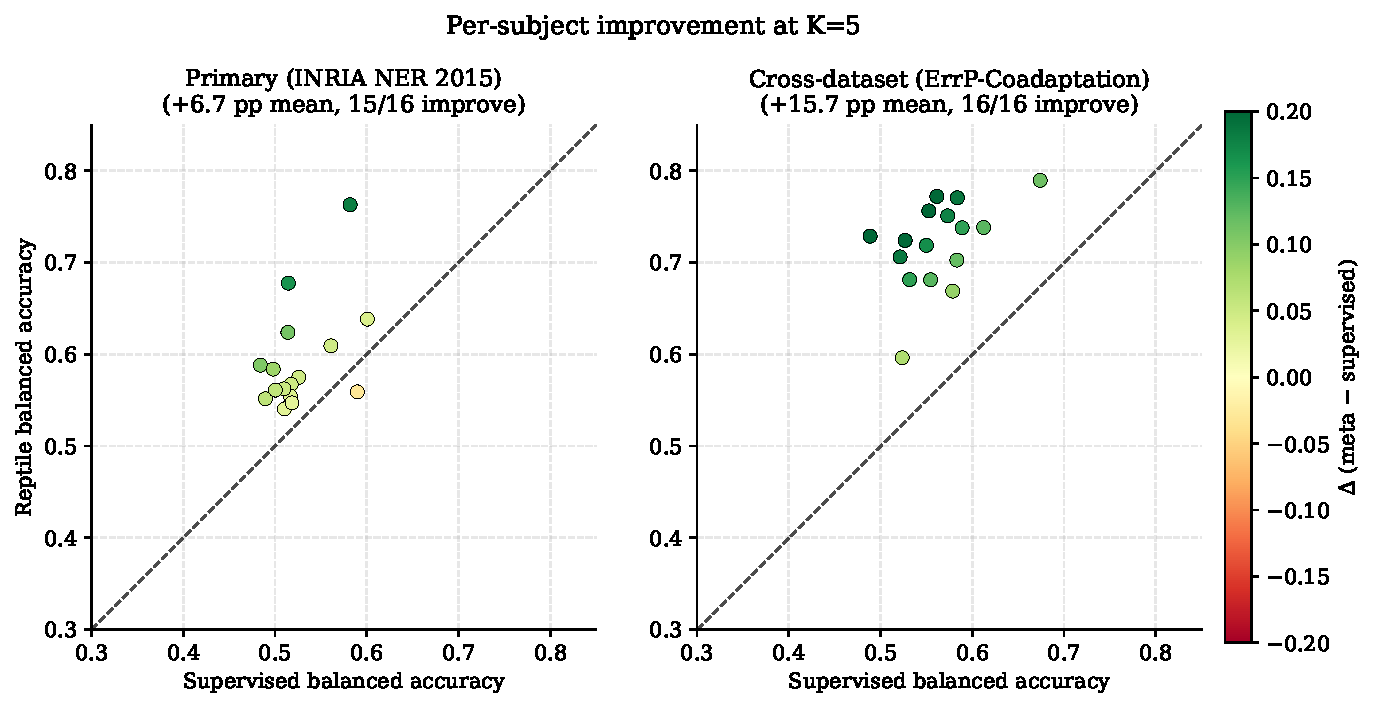
\includegraphics[width=\columnwidth]{figures/fig5_responder_scatter.pdf}
\caption{Per-subject balanced accuracy at $K{=}5$: Reptile vs.\ supervised.
Points above the diagonal are subjects where meta-learning helps; color encodes
the gain.}
\label{fig:responder}
\end{figure}

% ===================================================================
\section{Ablations}
Which design choices actually carry the result? Fig.~\ref{fig:ablation} isolates
three of them on the primary dataset.
\textbf{Class-weighted vs.\ uniform episodic loss.} This is the most impactful
choice. Weighting the loss by inverse class frequency lifts Full-MAML balanced
accuracy by 2--3 points and prevents the model from collapsing onto the majority
(correct) class---a real risk given the 75/25 split.
\textbf{FiLM vs.\ no-FiLM.} FiLM conditioning gives a small but significant gain at
$K{=}5$ ($+1.5$\,pp; paired Wilcoxon, $N{=}16$, $p{=}0.009$, $r{=}0.65$) that
disappears by $K{=}10$ ($p>0.27$; Fig.~\ref{fig:ablation}b). It is thus a minor,
low-shot-specific contributor rather than a primary driver.
\textbf{Feature dimensionality (32 vs.\ 128 PCA components).} Quadrupling the PCA
rank of the flattened waveform from 32 to 128 components did not improve the
meta-learners, indicating that 32 components already capture the discriminative
ErrP morphology and that the aggressive compression is not the bottleneck.

\begin{figure*}[t]
\centering
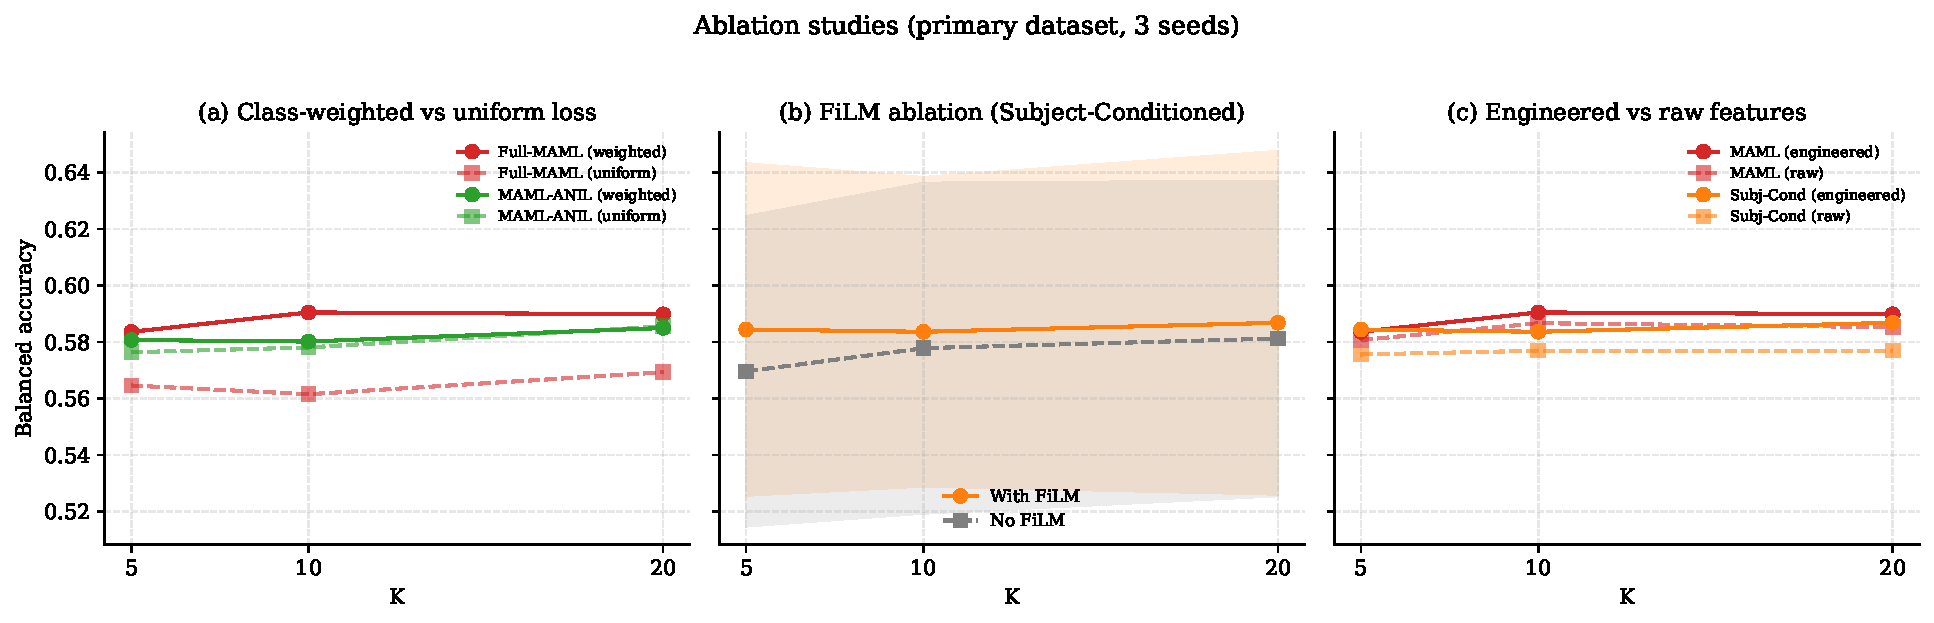
\includegraphics[width=\textwidth]{figures/fig4_ablations.pdf}
\caption{Ablations (primary dataset, three seeds). (a) class-weighted vs.\
uniform loss; (b) FiLM vs.\ no-FiLM in the subject-conditioned encoder;
(c) 32 vs.\ 128 PCA components.}
\label{fig:ablation}
\end{figure*}

% ===================================================================
\section{Discussion}
Two factors drive the few-shot gains: class-weighted episodic loss, which prevents
majority-class collapse under the 75/25 ErrP imbalance, and cross-subject
pre-training that produces a backbone from which only the classifier head needs
personalizing. This is consistent with the analysis of Raghu et al.~\cite{raghu2020rapid}:
MAML-ANIL (head-only adaptation) matches Full-MAML throughout our experiments
(0.581 vs.\ 0.584 at $K{=}5$ primary; 0.717 vs.\ 0.716 at $K{=}5$ validation),
indicating that the shared backbone is the key mechanism and full inner-loop
adaptation over the feature extractor adds little.

The results should be interpreted with their scope in mind. The meta-learners'
advantage over the strongest neural reference (EEGNet) is confined to the
five-trial regime on the cross-dataset paradigm: there they beat EEGNet by 6--7
points, but the gap closes by $K{=}10$ and reverses by $K{=}20$ (EEGNet 0.749),
and on the primary dataset they only match EEGNet at $K{=}5$ before EEGNet pulls
ahead. Meta-learning's practical niche is therefore narrow---the extreme low-data
regime, most clearly when generalizing across paradigms. The covariance-based
methods consistently fail at small $K$ on both datasets, consistent with their
need for well-conditioned covariance estimates.

Access to source-subject data does not by itself explain the gains. The
meta-learners outperform two transfer baselines (Pretrain-FT, Pretrain-ZeroShot)
that pretrain on the same source subjects with the same class-weighted loss, on
both datasets and at every shot count. Because these controls are matched on data
access and class weighting---the latter being the dominant ablation factor---the
residual gap isolates the episodic meta-objective rather than data volume or
imbalance handling.

\textbf{Statistical vs.\ practical significance.} A significant improvement is not
the same as a usable decoder. On the primary dataset the best methods reach only
$\sim$0.60 balanced accuracy at $K{=}5$---well above the 0.527 from-scratch
baseline in relative terms, but far from a deployable single-trial ErrP detector,
which for closed-loop correction would need both high error-class recall and low
false-alarm rates at an operating threshold. The cross-dataset numbers
($\sim$0.72) are more encouraging but still short of deployment. We therefore frame
the contribution as evidence that meta-learning improves low-data personalization,
not as a claim of deployment readiness; cost-sensitive thresholding and online
evaluation are needed before practical use.

\textbf{Limitations.} All experiments are offline simulations; we do not
demonstrate real-time closed-loop ErrP correction. We evaluate on two datasets and
a single backbone family (3-layer MLP / EEGNet variants) across three seeds;
additional ErrP datasets, larger or pretrained EEG backbones, and more seeds would
further strengthen the benchmark.

% ===================================================================
\section{Conclusion}
On two independent ErrP paradigms, gradient-based meta-learning, a
FiLM-conditioned encoder, and a source-pretrained EEGNet all significantly improve
over a from-scratch supervised baseline in the five-trial calibration regime.
On the cross-dataset validation at $K{=}5$, the gradient meta-learners additionally
outperform EEGNet by 6--7 percentage points, with seed-robust effects and broad
per-subject coverage (15--16 of 16 subjects improve); this edge over EEGNet is,
however, specific to $K{=}5$ and does not hold at $K{=}10$--$20$. The main design
lesson is that class-weighted episodic loss matters more than architecture, and
head-only adaptation (ANIL) matches full inner-loop MAML throughout. Against
transfer baselines matched on both source-data access and class weighting, the
meta-learners still win, locating the gain in the episodic meta-objective. The
absolute accuracies ($\sim$0.60 primary, $\sim$0.72 validation at $K{=}5$) are not
yet deployment-grade; future work should extend to additional ErrP datasets,
add cost-sensitive thresholding, and validate in a closed-loop online setting.

% ===================================================================
\bibliographystyle{IEEEtran}
\bibliography{references}

\end{document}
